\chapter{相关理论基础}
本章对论文中所涉及到的相关理论基础进行了介绍。首先介绍了注意力机制与Transformer模型架构,其次对Transformer模型在图表示学习领域中的应用进行了概述,最后对不同类型的知识图谱嵌入方法的核心思想和数学公式进行了说明,包括传统的知识图谱嵌入方法、基于图神经网络的知识图谱嵌入方法、基于图路径的知识图谱嵌入方法以及基于Transformer的知识图谱嵌入方法。

\section{注意力机制与Transformer网络}
深度学习中的注意力机制(Attention Mechanism)灵感来源于人类的视觉和认知系统。在推理过程中,注意力机制动态地为输入数据分配不同的权重,使模型能够自动地学习并选择性地关注输入中的重要信息,提高模型的性能和泛化能力。注意力机制最早被用于处理计算机视觉任务,后来在多个领域中得到了应用,例如自然语言处理和推荐系统等。

谷歌的研究团队于2017年提出的Transformer\upcite{Transformer}网络则是注意力机制方面里程碑式的工作。Transformer网络设计之初主要用于处理序列数据,在Transformer出现之前,序列数据的处理通常依赖于循环神经网络(RNN)及其变体,例如长短期记忆网络(LSTM)和门控递归单元(GRU)。RNN及其变体在处理序列数据时能够保持一定程度的历史信息,但存在一定的问题:由于对序列数据进行逐步处理,RNN在训练过程中容易出现梯度消失或者梯度爆炸的问题,特别是在处理长序列数据时。逐步处理也限制了模型的并行计算能力,导致训练效率低下。此外,尽管LSTM和GRU通过特殊的门控机制改善了长距离依赖问题,但当序列长度过高时,模型依然难以捕捉到距离较远的依赖关系。

Transformer\upcite{Transformer}网络通过使用自注意力(Self-Attention)机制解决了上述问题,在自注意力机制中,输入数据中的任意一个位置都能够直接感知到其它位置的信息,因此相比于传统的RNN结构,自注意力能够更加直接地捕捉到序列中长距离的依赖关系;自注意力机制允许模型在处理数据时并行计算各个位置的注意力分数,与RNN逐步计算的方式相比,可以显著提高模型的计算效率;自注意力机制通过学习输入序列中不同位置之间的动态相关性,能够根据特定的任务自适应地调整注意力分布。

Transformer\upcite{Transformer}网络中的自注意力机制的核心为缩放点积注意力机制,结构如图\ref{DotProductAttention}所示。
\begin{figure}[htbp]
  \vspace{-0.8cm}
  \centerline{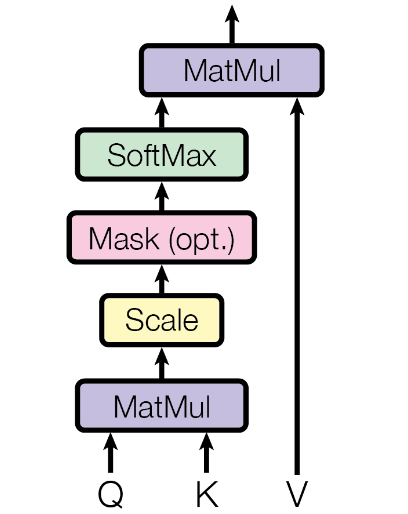
\includegraphics[width=0.250\textwidth]{pic/DotProductAttention.png}}
  \caption{缩放点积注意力机制}
  \label{DotProductAttention}
\end{figure}

具体来说,假设模型的输入为$X$,首先模型将会通过线性变化生成输入对应的查询向量$Q$,键向量$K$以及值向量$V$:
\begin{gather}
    Q=XW^Q, K=XW^K, V=XW^K
\end{gather}
其中$W^Q$、$W^K$、$W^K$是可学习的参数矩阵。

随后模型会将查询向量$Q$和键向量$K$进行点积并乘以缩放因子$\frac{1}{\sqrt{d_k}}$获得注意力分数,将其进行归一化处理转化为概率分布,用作权重对值向量$V$进行加权平均和,最终得到缩放点积注意力机制对应的输出,其中$d_k$为键向量的维度:
\begin{gather}
    \mbox{Attention}(Q,K,V) = \mbox{softmax}(\frac{QK^T}{\sqrt{d_k}})V
\end{gather}


进一步的,为了让模型能够同时关注来自不同维度的信息,并稳定自注意力的学习过程,Transformer采用了多头注意力机制,通过不同的参数矩阵将$Q$、$K$、$V$映射到不同的向量空间下并计算缩放点积注意力,将结果进行拼接获得最终的输出,如图\ref{MultiHeadAttention}所示。

具体来说,对于$h$个独立的注意力头,有:
\begin{equation}
  \begin{aligned}
    \mbox{MultiHead}(Q,K,V)&=\mbox{Concat}(head_1,...,head_h)W^O\\
    \mbox{where} \  head_i &=\mbox{Attention}(QW^Q_i,KW^K_i,VW^V_i)
  \end{aligned}
\end{equation}
其中$QW^Q_i$、$KW^K_i$、$VW^V_i$为将$Q$、$K$、$V$映射到第$i$个向量空间的参数矩阵,Concat为拼接操作。

\begin{figure}[htbp]
  \centerline{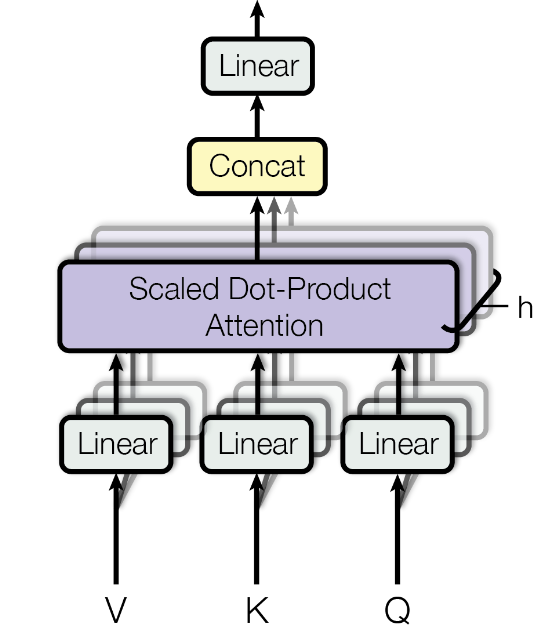
\includegraphics[width=0.3\textwidth]{pic/MultiHeadAttention.png}}
  \caption{多头注意力机制}
  \label{MultiHeadAttention}
\end{figure}
\section{基于Transformer的图表示学习方法}

图被广泛用于连接数据的网络结构表示,在社交系统、生态系统、生物网络、知识图谱等领域中都有广泛的应用。图表示学习方法将图的特征转化为低维嵌入空间中的向量。由于Transformer\upcite{Transformer}在计算机视觉和自然语言处理等领域展现出了出色的性能,近来,已经有大量的基于Transformer的模型被用于编码图结构数据。GraphTrans\upcite{GraphTrans}利用Transformer的自注意力机制学习图中的长距离的成对关系,并设计了一种读出机制以获得全局图嵌入。Grover\upcite{Grover}设计了节点级、边级和图级的自监督任务,能够从未标记的数据中学习图的结构和语义信息。Graphormer\upcite{Graphormer}对Transformer的注意力计算方式进行了改造,并从数学上证明了许多流行的图神经网络变体可以被视为Graphormer的特殊情况。

Graphormer\upcite{Graphormer}认为Transformer设计之初是为了建模序列数据,为了让其能够在图结构上实现最好效果,关键是要将图的结构信息恰当的融合到模型之中。Graphormer结合了几种有效的结构编码方法来利用这些信息。

Graphormer\upcite{Graphormer}认为Transformer模型中的注意力机制会基于节点的语义相似度计算注意力分布,因此提出了基于节点的出度和入度中心性编码来捕获知识图谱的节点重要性,其中$x_i$是节点表征,$z^-_{deg^-(v_i)}$和$z^+_{deg^+(v_i)}$是代表节点出度和入度的可学习表征:
\begin{equation}
  h_i^{(0)}=x_i+z^-_{deg^-(v_i)}+z^+_{deg^+(v_i)}
\end{equation}
Transformer模型在处理长序列文本时,会通过位置编码来学习文本之间的相对位置信息,但图不是序列数据,因此需要重新设计空间编码,加入到注意力运算中:
\begin{equation}
  A_{ij}=\frac{(h_iW_Q)(h_jW_K)^T}{\sqrt{d}}+b_{\varPhi (v_i,v_j)}
\end{equation}
这种编码方式的优势在于$b_{\varPhi (v_i,v_j)}$提供了一个对于图中的每个节点的全局的空间信息。

关系信息对于图中的节点表征至关重要,Graphormer\upcite{Graphormer}模型为了将关系信息加入到注意力中,引入了关系编码$c_{ij}$,表示的是节点$v_i$和$v_j$之间最短路径上所有关系表征的平均值,如下图公式所示:
\begin{equation}
  A_{ij}=\frac{(h_iW_Q)(h_jW_K)^T}{\sqrt{d}}+b_{\varPhi (v_i,v_j)}+c_{ij},\ \mbox{where} \ c_{ij} = \frac{1}{N}\sum_{n=1}^Nx_{e_n}(w_n^E)^T
\end{equation}
\section{知识图谱嵌入方法}

\subsection{传统的知识图谱嵌入方法}

传统知识图谱嵌入方法的研究对象是知识图谱中独立的三元组,集中于利用嵌入空间中的显式几何特性来捕捉实体之间的不同关系,基于翻译的方法、基于张量分解的方法和神经网络中的基于多层神经网络的、基于卷积神经网络的方法均属于此类。

基于翻译和基于张量分解的表示学习属于较早被提出的方法,它们模型结构简单,没有神经网络结构,计算速度快,可解释性较高。因此,在各个领域中的应用都十分广泛。

TransE\upcite{TransE}模型于2013年被提出,是基于翻译的知识图谱嵌入方法的起源。TransE的核心思想是将图谱中的关系视为嵌入空间内实体到实体的翻译,具体来说,TransE将实体和关系投影到相同的向量空间中,对于正确的事实三元组$(h,r,t)$,头实体嵌入$\boldsymbol{h}$和关系嵌入$\boldsymbol{r}$的相加结果应该尽可能得接近尾实体嵌入$\boldsymbol{t}$,即:
\begin{equation}
  \boldsymbol{h}+\boldsymbol{r}\approx \boldsymbol{t}
\end{equation}

而在TransE\upcite{TransE}的训练和评估过程中,对于训练集中的每一个正样本事实三元组$(h,r,t)$,TransE会通过随机替换头尾实体的方式,生成对应的负样本参与训练,这样的策略也成为了后续许多知识图谱嵌入方法的训练和评估策略。最终,对于扩充后的训练集中的每一个三元组$(h,r,t)$,TransE模型会计算$\boldsymbol{h}+\boldsymbol{r}$和$\boldsymbol{t}$之间的距离的L2范数作为衡量标准:
\begin{equation}
  d_r(h,t)=\left\lVert \boldsymbol{h}+\boldsymbol{r} - \boldsymbol{t}\right\rVert 
\end{equation}
对于正样本,TransE\upcite{TransE}期望得到的距离尽可能得小,负样本得到的距离尽可能的大,最终得到TransE模型的损失函数:
\begin{equation}
  \mathcal{L} =\sum_{(h,r,t)\in S}\sum_{(h^\prime,r,t^\prime)\in S^\prime_{(h,r,t)}}\left[\gamma +d_r(h,t)-d_r(h^\prime,t^\prime)\right] 
\end{equation}
其中$S$代表正样本集,$S^\prime_{(h,r,t)}$为生成的对应的负样本集。TransE方法最大的缺点是对复杂关系建模效果不佳,例如一对多、多对一以及多对多关系,容易把不同实体学习成相近的嵌入,随后的一系列基于翻译的方法针对这个缺点提出了很多的改进方式。

在基于张量分解的方法中,最为经典的是RESCAL\upcite{RESCAL}方法。给定一个知识图谱,RESCAL将其形式化为一个三阶张量${\mathcal{X} \in \mathbb{R}^{N \times N \times M}}$ ,其中$N$是实体的数量,$M$为关系种类的数量,张量的每一个切片$\mathcal{X}_k$对应于第$k$种关系的邻居矩阵,代表知识图谱中该种关系下实体之间的连接情况,如果实体$i$与实体$j$之间存在关系$k$,那么$\mathcal{X}_{ijk}$的值为1,否则为0。

RESCAL\upcite{RESCAL}假设每个实体$i$都可以通过一个向量$a_i \in \mathbb{R}^R$来表示,每类关系$k$由一个二维矩阵$R_k \in  \mathbb{R}^{R \times R}$表示,其中$R$为预定义的嵌入维度。RESCAL通过以下公式对张量$\mathcal{X}$进行分解:
\begin{equation}
  \mathcal{X}_k \approx A R_k A^T, \ \mbox{for} \ k=1,\ldots, m
\end{equation}
其中$A = [a_1,\ldots,a_N]$是实体嵌入矩阵。

RESCAL\upcite{RESCAL}模型的训练目标是最小化张量$\mathcal{X}$与通过学习到的实体和关系表示重建的张量之间的差异,因此模型的损失函数为:
\begin{equation}
  \min_{A,R_k} = f(A,R_k)+g(A,R_k)
\end{equation}
其中有:
\begin{equation}
  f(A,R_k)=\frac{1}{2}\left(\sum_k \left\lVert \mathcal{X}_k - AR_kA^T\right\rVert^2_F \right) 
\end{equation}
$g$为模型的正则项:
\begin{equation}
  g(A,R_k)=\frac{1}{2}\lambda \left(\left\lVert A\right\rVert^2_F+\sum_k\left\lVert R_k\right\rVert^2_F  \right) 
\end{equation}
其中$\left\lVert \cdot \right\rVert _F $为Frobenius范数,$\lambda$为正则化参数,用于防止过拟合。RESCAL\upcite{RESCAL}首次提出了基于张量分解的知识图谱嵌入方法,但也存在缺陷,用二维矩阵表示关系的方法使得RESCAL在处理大规模知识图谱时的计算成本和存储需求可能非常巨大,因此后续提出的一系列基于张量分解的方法在RESCAL的基础上进行了改进。

早期的基于神经网络的方法主要是采用多层神经网络来尝试直接拟合知识图谱。NTN\upcite{NTN}模型是一种用于知识图谱嵌入的神经网络架构,于2013年被提出。NTN通过引入张量运算和多层神经网络进行非线性特征变换来学习实体关系的语义信息,提高了模型的表达能力,克服了之前的知识图谱嵌入方法的限制。

NTN\upcite{NTN}模型采用低维向量代表实体,实体之间的关系则用一个三维张量进行表示。和RESCAL\upcite{RESCAL}模型类似,NTN引入了双线性张量操作。它通过在实体之间进行张量运算来捕捉实体之间的复杂交互关系,但是在NTN中还使用了基于多层神经网络的框架,相比于RESCAL,提供了更加丰富的线性特征表达能力。

在训练和评估过程中,NTN\upcite{NTN}通过以下公式来对事实三元组进行打分:
\begin{equation}
  f(h,r,t) = u_r^T \tanh\left(v_h^T M_r v_t + W_r^1v_h + W_r^2v_t + b_r\right) 
\end{equation}
其中,$v_h$和$v_t$分别为头实体和尾实体的嵌入向量,$u_r$为关系$r$的权重向量,$M_r$为关系$r$对应的三维张量,$W_r^1$和$W_r^2$为多层神经网络对应的线性变换矩阵,$b_r$为偏置项,$\tanh$为引入非线性的双曲正切激活函数。此外,NTN还采用了预训练的词向量来对实体和关系嵌入进行初始化,提升了模型的效果。

而随着卷积神经网络在计算机视觉领域大获成功,在知识图谱嵌入领域中也涌现出了以ConvE\upcite{ConvE}为代表的基于卷积神经网络的知识图谱嵌入方法。ConvE将设计和关系的嵌入表示重塑为二维矩阵,并用卷积神经网络来捕获实体和关系之间的复杂交互。具体来说,ConvE模型的具体计算步骤如下:

首先,对于给定的头实体$h$和关系$r$,ConvE\upcite{ConvE}将它们的嵌入重塑为二维形式,并拼接成一个二维矩阵:
\begin{equation}
  \left[\overline{\boldsymbol{h}};\overline{\boldsymbol{r}}\right] 
\end{equation}
其中$\left[;\right]$表示拼接操作,$\overline{\boldsymbol{h}}$和$\overline{\boldsymbol{t}}$表示头实体嵌入$\boldsymbol{h}$和关系嵌入$\boldsymbol{t}$重塑后的二维形式。

接下来ConvE\upcite{ConvE}对得到的二维矩阵进行卷积操作,应用ReLU激活函数$f$后得到的特征图为:
\begin{equation}
  f\left(\left[\overline{\boldsymbol{h}};\overline{\boldsymbol{r}}\right]\ast \omega\right)
\end{equation}
其中$\ast$表示卷积操作。随后ConvE将卷积层得到的特征图进行向量化,将得到的向量经过全连接层和ReLU激活函数后,形成最终的特征表示:
\begin{equation}
  f\left(\mbox{vec}\left(f\left(\left[\overline{\boldsymbol{h}};\overline{\boldsymbol{r}}\right]\ast \omega\right)\right)W\right)
\end{equation}
在预测阶段,模型将得到的特征表示与每个候选尾实体的嵌入进行点积得到对应的相似度得分:
\begin{equation}
  \psi_r(\boldsymbol{h},\boldsymbol{t})=f\left(\mbox{vec}\left(f\left(\left[\overline{\boldsymbol{h}};\overline{\boldsymbol{r}}\right]\ast \omega\right)\right)W\right)\boldsymbol{t}
\end{equation}
其中$\boldsymbol{t}$为尾实体嵌入。

最后,ConvE\upcite{ConvE}模型采用交叉熵损失函数对模型进行训练:
\begin{equation}
  \mathcal{L} (p,t)=-\frac{1}{N}\sum_i(t_i\cdot \log (p_i)+(1-t_i)\cdot\log(1-p_i))
\end{equation}
其中$p$为事实三元组正确的概率,有:
\begin{equation}
  p=\mbox{sigmoid}(\psi_r(\boldsymbol{h},\boldsymbol{t}))
\end{equation}

\subsection{基于图神经网络的知识图谱嵌入方法}
基于图神经网络的知识图谱嵌入方法是近些年知识图谱嵌入领域的一个重要发展方向,这类方法主要利用图神经网络的能力来学习图谱中实体和关系的嵌入表示。相比于传统的知识图谱嵌入方法,图神经网络天然适合处理图结构类型的数据,通过聚合一个实体周围的邻居节点信息来学习中心嵌入,这一过程能够捕捉到图谱中的局部拓扑信息,从而能够更好地表达实体之间的关系。此外,传统的嵌入模型往往只能考虑直接的实体关系,而图神经网络可以通过多层网络堆叠来捕捉实体之间的多跳路径信息,从而实现对更远距离实体关系的建模。

R-GCN\upcite{R-GCN}第一个在知识图谱嵌入领域应用图神经网络的方法。传统的图卷积网络主要设计用来处理无向图或者单一关系类型的图,但是这种方法无法直接应用于知识图谱,因为其忽略了图谱中边上的多种关系类型信息。而R-GCN则将图卷积神经网络扩展到了可以处理具有多种关系类型的图数据。R-GCN为图谱中的每种关系类型引入了一个单独的权重矩阵,每个关系类型在聚合邻居信息时能产生不同的影响,从而能够学习到每种关系特定的模式。R-GCN还在知识图谱中为每个实体添加了一个特殊类型的自环边,允许每个节点保留自身的信息,自环边在更新节点表示时作为单独的一种关系处理,也有自己的权重矩阵。

R-GCN\upcite{R-GCN}整体为编码器-解码器架构,使用改造后的图卷积神经网络作为编码器,使用DistMult\upcite{DistMult}方法作为链路预测任务的解码器,使用softmax函数来作为实体分类任务的解码器。

具体来说,R-GCN\upcite{R-GCN}的传播层用数学公式表示如下:
\begin{equation}
  h_i^{l+1}=\sigma \left(\sum_{r\in\mathcal{R}}\sum_{j\in\mathcal{N}_i^r}\frac{1}{c_{i,r}}W_r^lh_j^l+W_0^lh_i^l  \right) 
\end{equation}
其中$h_i^{l+1}$是第$i$个节点在经过第$l+1$层传播层更新后的表示,$\mathcal{N}_i^r$是节点$i$通过关系$r$相连接的邻居节点集合,$c_{i,r}$是归一化因子,一般设置为$c_{i,r}=\left\lvert\mathcal{N}_i^r\right\rvert$。

获得聚合后的实体表示后,R-GCN\upcite{R-GCN}使用DistMult\upcite{DistMult}方法对三元组进行打分:
\begin{equation}
  f(s,r,o)=e_s^TR_re_o
\end{equation}

训练用的损失函数为:
\begin{equation}
  \mathcal{L} =-\frac{1}{(1+\omega )\left\lvert\hat{\varepsilon } \right\rvert } \sum_{(s,r,o,y)\in \mathcal{T} }y\log l(f(s,r,o))+(1-y)\log(1-l(f(s,r,o)))
\end{equation}
其中$\omega$为R-GCN为每个正样本生成的负样本数量。
后续提出的基于图神经网络的方法在R-GCN的基础上进行了改进,基本沿用了R-GCN的编码器-解码器架构。SACN\upcite{SACN}将实体的邻域划分为带权值的子图进行聚合。TransGCN\upcite{TransGCN}提出了两种基于翻译的思想的编码器,分别用于实数域和复数域。

受到注意力机制在计算机视觉领域和自然语言处理领域的成功的启发,还有一部分基于图神经网络的方法尝试融合注意力机制。KBGAT\upcite{KBGAT}首次将图注意力网络用于知识图谱嵌入任务,RGHAT\upcite{RGHAT}使用实体和关系分层的方式对邻居的注意力进行了细分。

RGHAT\upcite{RGHAT}采用了一个创新的层次化注意力机制来充分利用实体的本地邻域信息,主要分为两层:关系级注意力根据不同关系对于中心实体重要性的不同为实体的每个邻接关系分配不同的权重;实体级注意力在关系级注意力的基础上进一步评估每个关系下邻居实体的重要性并分配对应的注意力分数。

对于中心实体$h$,邻接关系$r$的关系级注意力$\alpha_{h,r}$的计算方式如下:
\begin{gather}
  \mathbf{a}_{h,r} = \mathbf{W}_1\left[\mathbf{h}\Vert \mathbf{v}_r\right]\\
  \alpha_{h,r}=\mbox{softmax}_r(\mathbf{a}_{h,r})=\frac{\mbox{exp}(\sigma (\mathbf{p}\cdot \mathbf{a}_{h,r}))}{\sum_{r\prime \in \mathcal{N}_h }\mbox{exp}(\sigma(\mathbf{p}\cdot\mathbf{a}_{h,r^\prime}))}
\end{gather}
其中$\mathbf{h}$为实体$h$的嵌入,$\mathbf{W}_1$、$\mathbf{v}_r$和$\mathbf{p}$为可训练的参数,其中$\mathbf{v}_r$是关系特定的。

在关系级注意力的基础上,RGHAT进一步计算邻居节点$t$在关系$r$下对于中心实体$h$的实体级注意力$\beta_{r,t}$:
\begin{gather}
  \mathbf{b}_{h,r,t} = \mathbf{W}_2\left[\mathbf{a}_{h,r}\Vert \mathbf{t}\right]\\
  \beta_{r,t} = \mbox{softmax}_t(\mathbf{b}_{h,r,t}) = \frac{\mbox{exp}(\sigma(\mathbf{q}\cdot\mathbf{b}_{h,r,t}))}{\sum_{t\prime \in \mathcal{N}_{h,r}}\mbox{exp}(\sigma(\mathbf{q}\cdot \mathbf{b}_{h,r,t\prime}))} 
\end{gather}

之后将关系级注意力与实体级注意力相乘,RGHAT得到$(h,r,t)$在所有邻居三元组中的注意力得分$\mu_{h,r,t}$:
\begin{equation}
  \mu_{h,r,t} = \alpha_{h,r} \cdot \beta_{r,t}
\end{equation}

获得注意力得分之后,RGHAT\upcite{RGHAT}在每一层中对邻居信息进行聚合,结合中心实体自身的嵌入得到该层的输出:
\begin{gather}
  \hat{\mathbf{h}} = \sum_{r\in \mathcal{N}_h } \sum_{t\in\mathcal{N}_{h,r}}\mu_{h,r,t}\mathbf{b}_{h,r,t}\\
  \mathbf{h}^{'}  = \frac{1}{2}\left(\sigma(\mathbf{W}_3(\mathbf{h}+\hat{\mathbf{h}}))+\sigma(\mathbf{W}_4(\mathbf{h}\odot\hat{\mathbf{h}}))\right)
\end{gather}

RGHAT\upcite{RGHAT}还采用了多头注意力机制:
\begin{equation}
  \mathbf{h}^{'}=\mathop{\Vert}\limits_{k=1}^{K}\mathbf{h}^{'}_k
\end{equation}

通过采用层次化的注意力机制,RGHAT能够更精细地对实体的邻域进行建模,不仅聚焦于关系的重要性,还考虑了实体之间的语义贡献,提供了模型的可解释性。

基于图神经网络的方法通过图神经网络学习到了知识图谱的图结构信息,模型性能相比于之前的方法获得了明显的提升。但是这类方法依然存在一定的缺陷。一方面图神经网络采用的聚合邻居信息的方法比较简单,使得模型的表达能力受到了一定的限制;另一方面,基于图神经网络的方法主要是基于中心实体的局部邻域进行知识图谱补全,想要学习多跳之外的邻居信息就需要进行多层网络的堆叠,这会导致模型遭遇过度平滑问题,在学习图谱中长距离依赖方面存在较大的困难。
\subsection{基于图路径的知识图谱嵌入方法}

和基于图神经网络的方法利用中心实体的局部邻域进行链路预测不同,基于图路径的方法则尝试学习图谱中的路径信息来捕获实体与实体之间的长距离依赖,PTransE\upcite{PTransE}、RSN\upcite{RSN}和Interstellar\upcite{Interstellar}模型均属于此类,其中PTransE是其中较早的方法。

PTransE\upcite{PTransE}建立在TransE\upcite{TransE}模型的基础上,并增加了考虑实体间多步关系路径的能力。PTransE的主要贡献在于它不仅仅考虑实体之间的直接关系,还考虑通过其他实体间接连接的路径,从而捕获更丰富的语义信息。

在PTransE中,路径由一系列关系构成,定义为:
\begin{equation}
  \mathbf{p} = \mathbf{r}_1\circ \cdots \circ \mathbf{r}_l
\end{equation}
其中$\circ$表示关系的串联。PTransE\upcite{PTransE}模型尝试学习路径$\mathbf{p}$的表示,可以通过多种方式实现,例如通过关系向量的相加、乘积或者利用循环神经网络来进行学习,目的是最小化以下距离函数:
\begin{equation}
  E(h,p,t)=\left\lVert \mathbf{p}-(\mathbf{t}-\mathbf{h})\right\rVert =\left\lVert \mathbf{p}-\mathbf{r}\right\rVert=E(p,r) 
\end{equation}

PTransE\upcite{PTransE}模型将直接关系和间接关系一同考虑,所以基于翻译的思想,以下距离函数也需要同时最小化:
\begin{equation}
  E(h,r,t)=\left\lVert \mathbf{h}+\mathbf{r}-\mathbf{t}\right\rVert 
\end{equation}
最终,PTransE\upcite{PTransE}模型的损失函数为:
\begin{equation}
  L(\mathbf{S})=\sum_{(h,r,t)\in \mathbf{S}}\left[L(h,r,t)+\frac{1}{Z}\sum_{p\in P(h,r)}R(p\vert h,t)L(p,r)\right] 
\end{equation}
其中$R(p\vert h,t)$为路径的置信度,$L(h,r,t)$和$L(p,r)$为基于间隔的损失函数:
\begin{equation}
  L(h,r,t)=\sum_{(h^{'},r^{'},t^{'})\in \mathbf{S}^-}\left[\gamma +E(h,r,t)-E(h^{'},r^{'},t^{'})\right]_+ 
\end{equation}
\begin{equation}
  L(p,r)=\sum_{(h,r^{'},t)\in \mathbf{S}^-}\left[\gamma +E(p,r)-E(p,r^{'})\right]_+
\end{equation}

通过结合直接关系和通过多步路径发现的间接关系,PTransE\upcite{PTransE}能够捕捉实体之间更为复杂的交互模式,从而提高知识图谱补全任务的性能。但是,PTransE没有考虑到路径中的实体信息,因此后面提出的基于路径的知识图谱补全方法对PTransE进行了改进。

基于图路径的知识图谱嵌入方法通过图路径信息学习到了知识图谱中的长距离依赖,但是由于忽略了实体丰富的邻域结构,模型的性能收到了很大的限制。
\subsection{基于Transformer的知识图谱嵌入方法}

基于Transformer\upcite{Transformer}的知识图谱嵌入方法的核心思路是利用Transformer强大的表达能力来挖掘图谱中的语义和结构信息,以学习知识图谱的嵌入表示。Transformer模型的自注意力机制能够有效地捕捉实体之间的复杂关系和交互。还可以通过在Transformer中集成额外信息进一步加强实体和关系的表示。代表方法有HittER\upcite{HittER}和Relphormer\upcite{Relphormer}。

Relphormer\upcite{Relphormer}是一种为知识图谱嵌入任务而设计的基于Transformer的神经网络架构。为了解决知识图谱中实体与关系节点的异构性,Relphormer把实体和关系均视为相同的节点,有$ V=\mathcal{E} \cup \mathcal{R}$为节点集合,其中$\mathcal{E}$为实体集合,$\mathcal{R}$为关系集合,并用邻接矩阵$\mathbf{A} \in\left\{0,1\right\}^{\left\lvert V\right\rvert\times \left\lvert V\right\rvert} $来表示节点之间的连接关系,事实三元组表示为:$\mathcal{T} =(v_s,v_p,v_o)$,中心节点的局部邻域为:
\begin{equation}
  \mathcal{T}_G = \mathcal{T}_c \cup \mathcal{T}_{context}, \ \mbox{where} \ \mathcal{T}_{context} =\left\{\mathcal{T}_i\in\mathcal{N} \right\} 
\end{equation}
由于Transformer是序列数据模型,Relphormer利用Triple2Seq算法对中心节点的局部邻域进行随机采样,抽取一部分邻接三元组并转化对应的为序列数据。

由于知识图谱是图结构,为了防止局部邻域转化为序列数据后损失知识图谱的结构信息,Relphormer\upcite{Relphormer}提出了一种结构强化的自注意力机制,当计算注意力分数时,额外添加一个偏差项:
\begin{equation}
  a_{ij}=\frac{(\mathbf{h}_i\mathbf{W}_Q)(\mathbf{h}_j\mathbf{W}_K)}{\sqrt{d}}+\phi (i,j)
\end{equation}
\begin{equation}
  \phi (i,j)=f_{structure}(\tilde{\mathbf{A}^1},\tilde{\mathbf{A}^2},\cdots,\tilde{\mathbf{A}^m} )
\end{equation}
其中$\tilde{\mathbf{A}}$是归一化后的邻接矩阵,$\tilde{\mathbf{A}^m}$是$\tilde{\mathbf{A}}$的$m$次方,指在$m$步内节点的连通性。

对于一些较为密集的知识图谱,每步训练中对局部邻域的随机采样过程随机性较大,可能会导致训练过程中的不一致性。为了避免这个问题,Relphormer利用上下文对比策略来克服不稳定性,使用不同训练步骤中相同三元组的采样的局部邻域的内容来强制模型进行类似的预测,最小化以下损失函数:
\begin{equation}
  \mathcal{L}_{contextual} = -\log\frac{\mbox{exp}(\mbox{sim}(\boldsymbol{c}_t,\boldsymbol{c}_{t-1})/\tau )}{\mbox{exp}(\mbox{sim}(\boldsymbol{c}_t,\boldsymbol{c}_{t-1})/\tau )+\sum_j\mbox{exp}(\mbox{sim}(\boldsymbol{c}_t,\boldsymbol{c}_{j})/\tau )}
\end{equation}
其中$\tau$为温度系数,$\boldsymbol{c}_t$为第$t$步采样到的样本的表示,$\mbox{sim}(\boldsymbol{c}_t,\boldsymbol{c}_{t-1})$为$\boldsymbol{c}_t$与$\boldsymbol{c}_{t-1}$之间的余弦相似度:$\frac{\boldsymbol{c}_t^T\boldsymbol{c}_{t-1}}{\left\lVert \boldsymbol{c}_{t}\right\rVert \cdot \left\lVert \boldsymbol{c}_{t-1}\right\rVert }$。

受掩码语言模型例如BERT\upcite{BERT}的启发,和之前的知识图谱嵌入方法不同,Relphormer\upcite{Relphormer}采用了一种新的训练策略:随机掩盖输入序列中的特定节点,然后对其进行预测。具体来说,在训练过程中,随机遮掩中心三元组头实体或者尾实体,并利用剩余的节点序列$\mathcal{T}_M$和上下文邻接矩阵$\mathbf{A}_G$的情况下,预测缺失的部分$Y$:
\begin{equation}
  \begin{aligned}
    &\mathcal{T}_M = MASK(\mathcal{T}_G)\\
    &Relphormer(\mathcal{T}_M,\mathbf{A}_G)\rightarrow Y
  \end{aligned}
\end{equation}

最终,Relphormer\upcite{Relphormer}模型的损失函数为:
\begin{equation}
  \mathcal{L}_{all} = \mathcal{L}_{MKM}+\lambda \mathcal{L}_{contextual}
\end{equation}
其中$\mathcal{L}_{MKM}$和$\mathcal{L}_{contextual}$分别为掩盖预测任务和上下文对比任务的损失函数。


\section{本章小结}

本章对论文中所涉及到的相关理论基础和关键技术进行了介绍,方便后续章节的说明。首先对注意力机制与Transformer模型的原理进行介绍,然后介绍了Transformer网络在图表示学习中的应用,最后介绍了知识图谱嵌入方法,包括不利用图结构的传统的知识图谱嵌入方法,以及基于图神经网络的知识图谱嵌入方法、基于图路径的知识图谱嵌入方法和基于Transformer的知识图谱嵌入方法。